\section{Cycles from frames and a dimension estimate}\label{sec:frames}

This section constructs a space of cycles from decompositions into lines.
Its dimension must remain large when the dimension of the underlying space
increases while the field stays fixed.  The estimate concerns coefficients
on subgroup flags, rather than the number of expressions of a chain as a
sum of apartments.  We first construct these coefficients and then estimate
their dimension using a Lie superalgebra.

The proof has three stages. Boundary cancellation produces the cycles,
and merger coefficients identify the space whose dimension must be
estimated. The supporting-subspace grading then permits a PBW count
without forgetting where a coefficient is supported. Finally, the
relation kernel and its marked-factor inequality reduce the estimate
to explicit plane counts. Each stage retains the actual flag
coefficients needed in the later restriction and propagation arguments.

\subsection{Frames, sign flags, and the statement}

Fix one of the following structures:
\begin{enumerate}
\item vector spaces over $\F_u$, with all lines allowed;
\item nondegenerate hermitian spaces over $\F_{u^2}$, with all
nondegenerate lines allowed;
\item nondegenerate symmetric spaces over $\F_u$, where $u$ is odd,
with both square classes of nondegenerate lines allowed;
\item nondegenerate symmetric spaces over $\F_u$, where $u$ is odd,
with only one specified square class of nondegenerate lines allowed.
\end{enumerate}
All direct sums in a form space are required to be orthogonal.  In the
fourth case an admissible space means a space isometric to a sum of allowed
lines.  In the other cases every space with the indicated structure is
admissible.  A \emph{frame} of an admissible space $W$ is an unordered
decomposition $\mathcal D=\{L_1,\ldots,L_h\}$ into allowed lines, where
$h=\dim W$.  Write $\mathfrak F(W)$ for its set of frames.  An ordered
frame will also be called a word, and written $L_1\cdots L_h$.

For any prime $p$, attach to a frame its abstract projective sign space
\[
 S(\mathcal D)=\F_p^{\mathcal D}/\langle(1,\ldots,1)\rangle.
\]
It is an elementary abelian group of rank $h-1$.  A partition $\pi$ of
$\mathcal D$ specifies the subgroup on which the coordinates belonging to
each block of $\pi$ are equal.  This subgroup has rank $|\pi|-1$.
Two partitions give distinct subgroups: two coordinates belong to the
same block precisely when their difference vanishes identically on the
subgroup.  For coordinates in distinct blocks, assign the values $0$ and
$1$ to those blocks to distinguish them.  This argument works also for
$p=2$ and survives the quotient by simultaneous signs.

We make the identifications between different frames explicit.  Let
$\mathcal D(W)$ be the poset of decompositions of $W$ into at least two
nonzero admissible subspaces.  Put $\mathcal E\leq\mathcal E'$ when
$\mathcal E'$ refines $\mathcal E$.  Merging blocks in a frame therefore
gives the same vertex whenever it gives the same decomposition of $W$.
The flags from two blocks through a full frame have $h-1$ vertices and
dimension $h-2$.  At a fixed frame these are exactly the equal-sign flags
just described.

In the hermitian case, this is the proper orthogonal-decomposition
poset of \citet[Sections~2.1 and~7.2, arXiv version~2]{PitermanWelker2024},
with the order reversed. Their Proposition~7.3(i) relates eigenspace
decompositions to elementary subgroups and credits the corresponding
construction of \citet[pp.~514--515]{AschbacherSmith1993}.
The partial-frame complex is a different object. Here the full
coefficient space, and its dimension for each isometry type, are the
objects required for the subsequent chain construction.

For an ordered frame $w=L_1\cdots L_h$, let $r=h-1$ and set
$\lambda_i=x_i-x_{i+1}$ for $1\leq i\leq r$.  These functionals form a
basis of $S(\mathcal D)^*$.  For $\sigma\in\mathfrak S_r$, put
\[
 K_j(w,\sigma)=\bigcap_{a=1}^j\ker\lambda_{\sigma(a)}
 \quad(0\leq j\leq r),\qquad K_0(w,\sigma)=S(\mathcal D).
\]
The subgroups $K_j$ are also vertices of $\mathcal D(W)$ when $j<r$.
Define the coned apartment chain
\begin{equation}\label{eq:frame-apartment}
 a_w=\sum_{\sigma\in\mathfrak S_r}\sgn(\sigma)
 [K_{r-1}(w,\sigma)<\cdots<K_1(w,\sigma)<S(\mathcal D)]
 \in\widetilde C_{h-2}(\mathcal D(W);\Q).
\end{equation}
In dimension one the same convention gives the empty simplex in degree
$-1$.  This convention will occur only when describing a boundary of a
two-dimensional frame.

Let $V_{\mathcal D}$ be the span of the actual flag-coefficient vectors of
$a_w$ as $w$ runs over the orderings of $\mathcal D$.  Thus two linear
combinations with identical coefficients define the same member of
$V_{\mathcal D}$.  We will prove that
\begin{equation}\label{eq:local-frame-dimension}
 \dim V_{\mathcal D}=(h-1)!.
\end{equation}
An assignment is a member of $\bigoplus_{\mathcal D\in\mathfrak F(W)}
V_{\mathcal D}$.  Summing its components embeds this direct sum into the
chain space, since a full flag determines its top frame.

Here is the subspace of assignments that we use.  Let $f$ be a
$\Q$-valued function on ordered frames.  For every ordered decomposition
\[
 L_1\oplus\cdots\oplus L_{i-1}\oplus Q\oplus
 L_{i+2}\oplus\cdots\oplus L_h=W,
 \qquad \dim Q=2,
\]
with the other summands allowed lines, require
\begin{equation}\label{eq:frame-plane-relation}
 \sum_{(A,B):\,Q=A\oplus B}
 f(L_1\cdots L_{i-1}AB L_{i+2}\cdots L_h)=0.
\end{equation}
The sum is over all ordered allowed frames of $Q$, with orthogonality
understood in the form cases.  Define $\mathcal Z(W)$ to be the image of
all these functions under $f\mapsto\sum_w f(w)a_w$, viewed as an assignment
of actual coefficients.  The following theorem is uniform in the
isometry type of $W$.

\begin{theorem}[Frame coefficient bound]\label{thm:frame-bound}
Let $W$ have dimension $h\geq2$ and one of the four structures above,
and suppose that $W$ admits an allowed frame.  The space
$\mathcal Z(W)\subseteq\bigoplus_{\mathcal D\in\mathfrak F(W)}V_{\mathcal D}$
consists of cycles of degree $h-2$, each supported on full flags ending
at sign groups of rank $h-1$.  Moreover,
\begin{equation}\label{eq:frame-bound}
 \dim\mathcal Z(W)\ \geq\
 F_h\,|\mathfrak F(W)|(h-1)!.
\end{equation}
The following choices of $F_h$ are valid for each individual isometry
type of $W$.
\begin{enumerate}
\item In the no-form case over $\F_u$, and in the hermitian case over
$\F_{u^2}$, set
\[
 \rho=\frac1{u(u+1)}\quad\hbox{and}\quad
 \rho=\frac1{u(u-1)},
 \quad\hbox{respectively},\qquad
 y=\frac{1+\sqrt{1-4\rho}}2.
\]
For $u\geq5$ one may take $F_h=y^h+(1-y)^h\geq(17/25)^h$.
\item For a symmetric space over $\F_u$, with both line types allowed
and $u\geq5$ odd, put
\[
 x=\frac{1+\sqrt{1-4u/(u^2-1)}}2.
\]
One may take
\begin{equation}\label{eq:symmetric-frame-fraction}
 F_h=x^h+(1-x)^h-\mathbf1_{2\mid h}\,2(u^2-1)^{-h/2}
 \ \geq\ (17/25)^h.
\end{equation}
In particular $F_3\geq3/8$.
\item For a symmetric space over $\F_u$ with one fixed line type,
where $u\geq7$ is odd, write $\chi$ for the quadratic character of
$\F_u^\times$ and set
\[
 \rho=\frac2{u-\chi(-1)},\qquad
 y=\frac{1+\sqrt{1-4\rho}}2.
\]
One may take $F_h=y^h+(1-y)^h>0$.
\end{enumerate}
The same statements hold for any realization by projective sign
subgroups in which coarsened decompositions give the indicated subgroup
flags and the complete flags ending at the full frames remain distinct.
\end{theorem}

The last qualification states precisely what is required to carry the
abstract construction into a group.  Additional identifications of
boundary faces cause no difficulty, because their coefficients already
sum to zero.  An identification of full flags could decrease the
dimension; the applications will verify that this does not occur.

\subsection{Boundary cancellation and coefficient detection}

We first address the cycle assertion, then turn to coefficient detection.

The distinction between simplex coefficients and their boundary sums
is central to the constructible cycles of
\citet[Proposition~4.2 and Definition~4.3, arXiv version~1]{DiazRamos2018} and to
\citet[Proposition~3.2 and Theorems~3.3--3.5]{DiazRamosMazza2022}.
The plane relations below impose this distinction on frame flags.

For a word $w$ and a gap $i$, denote by $w/i$ the ordered decomposition
obtained by replacing $L_i,L_{i+1}$ by their sum.  The definition
\eqref{eq:frame-apartment} applies to this shorter list of blocks as well.
Deleting an interior vertex of an apartment flag has two contributions
whose permutations differ by transposing the two equations on either
side of that deletion.  Their signs are opposite.  This includes deletion
of the bottom vertex: in that case one transposes the last imposed
equation and the one omitted equation.  Only deletion of the cone vertex
$S(\mathcal D)$ remains.  Grouping its contributions according to the
first equation imposed gives the exact formula
\begin{equation}\label{eq:frame-apartment-boundary}
 \partial a_w=(-1)^{r-1}\sum_{i=1}^{r}(-1)^{i-1}a_{w/i}.
\end{equation}
Indeed, moving gap $i$ to the first position contributes $(-1)^{i-1}$,
and deletion of the final vertex of an increasing flag contributes
$(-1)^{r-1}$.  On $\ker\lambda_i$, the remaining equations are the
adjacent-difference equations of $w/i$ in their original order.  Formula
\eqref{eq:frame-plane-relation} now cancels each term of
\eqref{eq:frame-apartment-boundary} after summing with the weights $f(w)$.
If different coarsening descriptions give the same face, this only adds
several zero sums.  Consequently every member of $\mathcal Z(W)$ is a
cycle, including the augmented degree-zero assertion when $h=2$.

To determine the rank of the coefficient map, regard a line as a formal
letter of odd parity.  If homogeneous words or brackets $A,B$ have
parities $|A|,|B|\in\mathbb Z/2$, their supercommutator is
\begin{equation}\label{eq:frame-superbracket}
 [A,B]=AB-(-1)^{|A||B|}BA.
\end{equation}
In particular $[L,M]=LM+ML$ for two line letters.  A binary merger tree
on a frame defines an iterated bracket by choosing an order for the two
children of each internal vertex and using \eqref{eq:frame-superbracket}.
The parity of a subtree is its number of leaves modulo two.

This tree description is closely related to the multilinear
super-Lie model of \citet[Proposition~3.4, Corollary~3.5, and
Section~3.6]{Robinson2004}; see also
\citet[Theorem~7.3]{Stanley1982} for the partition representation.
We prove the coefficient formula with our coning and orientation
conventions. In particular, the chains here have degree $h-2$,
whereas the proper partition complex with both endpoints removed has
degree $h-3$.

\begin{lemma}[Merger coefficients]\label{lem:merger-coefficients}
For a full flag in $\mathcal D(W)$ ending at a frame $\mathcal D$, complete its sequence of
binary mergers by the final, implicit merger to the one-block partition.
Its coefficient in $\sum_w f(w)a_w$ is, up to one sign depending on the
flag and the chosen child orders, the evaluation of $f$ on the associated
iterated superbracket.  All iterated brackets on the letters of
$\mathcal D$ occur in this way.  Their span has dimension $(h-1)!$.
\end{lemma}

\begin{proof}
The words contributing to a specified flag are exactly the orders of
the leaves in which the leaves below every internal vertex form an
interval.  For each such word there is a unique order of the adjacent
gaps giving the specified mergers, including the final omitted gap.
Choose one compatible order of the leaves.  Every other compatible
order is obtained by independently interchanging the two child
intervals at internal vertices.

Suppose those intervals have $a$ and $b$ leaves.  There are $a-1$ gaps
internal to the first interval and $b-1$ internal to the second, besides
their separating gap.  Interchanging the intervals permutes their
internal gaps past each other and moves the separating gap past both
sets.  The resulting sign is
\[
 (-1)^{(a-1)(b-1)+(a-1)+(b-1)}
   =(-1)^{ab-1}=-(-1)^{ab}.
\]
This is exactly the change prescribed by the two terms of
$[A,B]$.  Expanding the bracket recursively therefore gives the
coefficient of the flag, with the sign of the initially chosen word as
a common factor.  Every binary tree admits an order of its internal
vertices in which children precede parents.  Such an order gives a full
flag of mergers, so every bracket occurs.

Fix one letter $L_0$.  Super skew-symmetry and the super Jacobi identity
\begin{equation}\label{eq:frame-jacobi}
 [X,[Y,Z]]=[[X,Y],Z]+(-1)^{|X||Y|}[Y,[X,Z]]
\end{equation}
span every bracket by left combs
\[
 [\cdots[[L_0,L_{i_2}],L_{i_3}],\ldots,L_{i_h}],
\]
where $(i_2,\ldots,i_h)$ orders the other letters.  To see the spanning
assertion inductively, first use skew-symmetry to place the subtree
containing $L_0$ on the left.  Expand that subtree by induction.
Applying \eqref{eq:frame-jacobi} repeatedly to any nontrivial right
subtree replaces it by brackets with smaller right subtrees.  Continue
until only single letters are appended; skew-symmetry puts the term
containing $L_0$ on the left whenever necessary.
There are $(h-1)!$ such combs.  Each comb has exactly one associative
word beginning with $L_0$, namely
$L_0L_{i_2}\cdots L_{i_h}$, with coefficient $1$.  This follows by
induction from \eqref{eq:frame-superbracket}: the term with the newly
appended letter first cannot start with $L_0$.  Distinct combs have
distinct such words, proving their independence.  The coefficient
functionals of the full flags span precisely this bracket space.
Their rank, and hence $\dim V_{\mathcal D}$, is $(h-1)!$.
\end{proof}

Figure~\ref{fig:merger-tree} illustrates a merger flag and its coefficient
bracket for four lines.

\begin{figure}[ht]
\centering
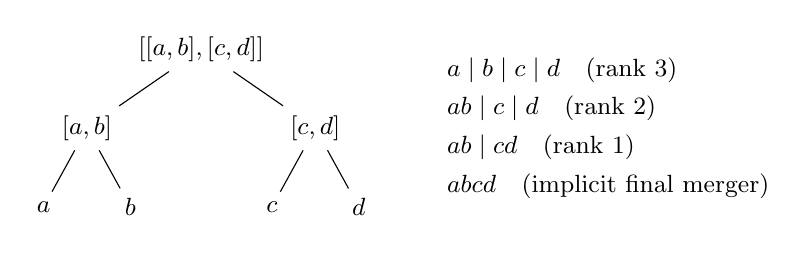
\begin{tikzpicture}[every node/.style={font=\small},level distance=12mm]
 \node (root) at (0,0) {$[[a,b],[c,d]]$};
 \node (ab) at (-1.45,-1) {$[a,b]$};
 \node (cd) at (1.45,-1) {$[c,d]$};
 \node (a) at (-2,-2) {$a$};
 \node (b) at (-.9,-2) {$b$};
 \node (c) at (.9,-2) {$c$};
 \node (d) at (2,-2) {$d$};
 \draw (root)--(ab)--(a) (ab)--(b) (root)--(cd)--(c) (cd)--(d);
 \node[align=left,anchor=west] at (3.0,-1)
 {$a\mid b\mid c\mid d$\quad(rank $3$)\\[3pt]
  $ab\mid c\mid d$\quad(rank $2$)\\[3pt]
  $ab\mid cd$\quad(rank $1$)\\[3pt]
  $abcd$\quad(implicit final merger)};
\end{tikzpicture}
\caption{A full flag of projective sign groups records binary mergers.
The left tree determines its coefficient functional.  The two children
at the root each have even parity, so interchanging them changes its
sign.  Interchanging the two leaves of either bottom pair does not.
The list is in merger order; the oriented subgroup flag has increasing
ranks $1,2,3$, with the implicit one-block merger omitted.}
\label{fig:merger-tree}
\end{figure}

The remaining task is quantitative.  Plane relations connect different
frames, so the local dimension $(h-1)!$ does not by itself give a lower
bound on the space of cycles.  We encode all these relations at once,
while retaining enough information to distinguish every supporting
subspace.

\subsection{The supporting-subspace grading and PBW}

Fix a finite ambient space $W_0$ of one of the permitted structures.
Form a commutative monoid with elements $0$, all its nonzero admissible
subspaces, and an additional element $\bot$.  For admissible subspaces
$A,B$, their sum in this monoid is the subspace $A\oplus B$ if they form
an allowed direct decomposition, and is $\bot$ otherwise.  Set
$\bot+A=\bot$, with $0$ an identity.  This operation is associative:
an iterated product avoids $\bot$ precisely when all its nonzero
subspaces form a direct decomposition, orthogonal when required.
Once directness or orthogonality fails, adjoining another summand cannot
restore it.  We call degrees other than $\bot$ \emph{good degrees}.

Let $V$ be the rational vector space with one odd generator $e_L$ for
each allowed line $L\leq W_0$, and give $e_L$ degree $L$.  Also retain
the usual word-length grading.  In the tensor algebra $T(V)$, a word
has good degree $X$ exactly when its letters are an ordered frame of
$X$; its length is then $\dim X$.  For each admissible plane $Q\leq W_0$
define
\begin{equation}\label{eq:frame-rq}
 r_Q=\sum_{(A,B):\,Q=A\oplus B}e_Ae_B
     =\sum_{\{A,B\}:\,Q=A\oplus B}[e_A,e_B].
\end{equation}
The second sum is over unordered frames and is independent of their
ordering, because the two generators are odd.  Each $r_Q$ is nonzero,
even, and homogeneous of good degree $Q$ and length $2$.

Let $\mathfrak L$ be the free Lie superalgebra on $V$, and let
\[
 P=\mathfrak L/(r_Q:Q\text{ an admissible plane})_{\Lie},\qquad
 U=T(V)/(r_Q:Q\text{ an admissible plane})_{\mathrm{ass}}.
\]
The subscripts mean the Lie ideal and the two-sided associative ideal,
respectively.  The universal properties show that $U$ is the enveloping
algebra of $P$: an associative-algebra map out of either presentation is
exactly a map on the line generators annihilating every $r_Q$.

We use the characteristic-zero super PBW theorem \cite{Scheunert1979};
the positive word-length graded form over $\Q$ is also given by
\citet[discussion following Proposition~5.2 and Theorem~5.16]{MilnorMoore1965}.
We use it
in the following explicit form.  For a homogeneous ordered basis of a Lie superalgebra,
its enveloping algebra has as a basis the ordered products of basis
elements, with each odd basis element used at most once.  Its associated
graded algebra for the number-of-factors filtration is
$\Sym(P_{\mathrm{even}})\otimes\bigwedge(P_{\mathrm{odd}})$.
The canonical map from the Lie superalgebra to its enveloping algebra
is consequently injective.  Recall why the parity qualification is
necessary: the relation for homogeneous elements is
$xy-(-1)^{|x||y|}yx=[x,y]$, and for odd $x$ it becomes
$2x^2=[x,x]$.  Ordering adjacent factors and replacing odd squares
therefore gives the stated normal forms.  The overlap of three
successive factors reduces to
\[
 [x,[y,z]]-[[x,y],z]-(-1)^{|x||y|}[y,[x,z]]=0;
\]
the overlaps with repeated odd factors are its specializations, using
$2x^2=[x,x]$ and $[x,[x,x]]=0$.  Thus these reductions are consistent
by super Jacobi.  Induction on factor length and then on the number of
out-of-order pairs gives the PBW normal forms.  This description also
shows that PBW preserves any additional grading for which the bracket
is homogeneous, including the supporting-subspace and length gradings
above.

Write $P(X)$ and $U(X)$ for the good components on a subspace $X$.
These are finite-dimensional and intrinsic to $X$.  Indeed, a product
of good degree $X$ uses only supports contained in $X$; an expression
of bad degree can never contribute to it.  Thus neither generators nor
relations supported outside $X$ affect that component.  We may
therefore form these spaces in any ambient space containing $X$.

In a good PBW monomial, the supports of its nonzero factors are
independent admissible subspaces.  In particular no basis factor can
occur twice, even when it is even.  The distinction between symmetric
and exterior multiplication changes signs but does not change the
number of such monomials.  We have proved a vector-space decomposition
in good degree:
\begin{equation}\label{eq:frame-pbw-decomposition}
 U(X)\ \cong\
 \bigoplus_{k\geq0}\ 
 \bigoplus_{X=X_1\oplus\cdots\oplus X_k\,/\,\mathfrak S_k}
 P(X_1)\otimes\cdots\otimes P(X_k),
\end{equation}
where all $X_i$ are nonzero, and the tensor factors on the right may
be ordered by any fixed order of their supports.  The term $k=0$
occurs only for $X=0$.

\begin{lemma}[Identification with coefficient assignments]
\label{lem:frame-lie-identification}
For every admissible $W$ of dimension at least two, the coefficient
construction has image of dimension $\dim P(W)$:
\[
 \dim\mathcal Z(W)=\dim P(W).
\]
\end{lemma}

\begin{proof}
The good component $T(V)(W)$ has the ordered frames as its basis.
The component of its defining ideal is spanned by all expressions
$a r_Q b$ of good degree $W$, where $a,b$ are words.  Being good forces
the outside letters and the plane $Q$ to form a direct decomposition.
Consequently their annihilator is exactly the space of functions
satisfying \eqref{eq:frame-plane-relation}.  That space is $U(W)^*$.

The good component of the free Lie superalgebra is spanned by brackets
whose letters form a frame: any other support is bad.  Its image in
$U(W)$ is $P(W)$, by PBW injectivity.  By
Lemma~\ref{lem:merger-coefficients}, the coefficient functionals of all
the full flags are precisely, up to signs and possible repetitions,
the evaluations on these brackets.  They span $P(W)$.  Restriction of
functionals $U(W)^*\to P(W)^*$ is surjective, because these spaces are
finite-dimensional.  The rank of the actual coefficient map is
therefore $\dim P(W)$, as asserted.
\end{proof}

\subsection{Normalized series and the relation kernel}

We now use formal series to count the good components in all dimensions.
Let $G_X$ be the full linear group of $X$ in the no-form case and the
full isometry group in the form cases, with $|G_0|=1$.  For any
isometry-invariant collection $M(X)$ of finite-dimensional vector
spaces, define
\[
 \mathsf M=\sum_{[X]}\frac{\dim M(X)}{|G_X|}\,[X].
\]
Here $[X]$ is a formal symbol for its isomorphism or isometry type,
and $[X][Y]=[X\oplus Y]$.  Series are completed by dimension, so each
coefficient in a product is a finite sum.  The coefficientwise order
always refers to this type basis.  If
\[
 (M*N)(W)=\bigoplus_{W=A\oplus B}M(A)\otimes N(B),
\]
then its series is $\mathsf M\mathsf N$.  To verify this, for specified
types $A,B$ the group $G_W$ acts transitively on the ordered
decompositions of these types, with stabilizer $G_A\times G_B$.
Transitivity follows by taking the direct sum of chosen isomorphisms
or isometries on the summands.  The number of decompositions is
$|G_W|/(|G_A||G_B|)$, which is exactly the normalization asserted.

Write $\mathsf P,\mathsf U$ for the series of $P,U$.  Dividing the
ordered versions of \eqref{eq:frame-pbw-decomposition} by $k!$ gives
\begin{equation}\label{eq:frame-exponential}
 \mathsf U=\exp(\mathsf P).
\end{equation}
There is no stabilizer correction beyond $k!$: the actual nonzero
summands of a direct decomposition are distinct, even if some of their
isometry types agree.  An ordering of a decomposition therefore has
exactly $k!$ possibilities.

Let $R$ be the vector space with one formal even basis element $\mathbf r_Q$
for each admissible plane $Q$, of degree $Q$.  Denote the series of
$V$ and $R$ by $v$ and $w$, respectively.  Split each relation just
before its last letter to define the left $U$-module map
\[
 d_2:U\otimes R\longrightarrow U\otimes V,
 \qquad
 d_2(u\otimes\mathbf r_Q)
   =\sum_{(A,B):Q=A\oplus B}u e_A\otimes e_B.
\]
Let $d_1:U\otimes V\to U$ be multiplication and put $C=\ker d_2$.
We have an exact sequence
\begin{equation}\label{eq:frame-relation-complex}
 0\longrightarrow C\longrightarrow U\otimes R
 \xrightarrow{d_2}U\otimes V\xrightarrow{d_1}U
 \longrightarrow\Q\longrightarrow0.
\end{equation}
Here is the only exactness assertion needing verification.  Write
$T=T(V)$ and let $I$ be the two-sided ideal generated by the $r_Q$.
Splitting the last letter identifies $T_+$ with $T\otimes V$ and
$U\otimes V$ with $T_+/(IV)$.  Hence the kernel of $d_1$ identifies
with $I/(IV)$.  Every element of $I$ is a sum of terms $a r_Q b$.
When $b$ has positive length this term lies in $IV$, by separating
the last letter of $b$.  The terms with $b=1$ are exactly the images
of $d_2$.  This proves exactness; $d_1$ plainly has image the
augmentation ideal.  These maps preserve the supporting-subspace
grading, so exactness holds in every good component.

Taking dimensions of \eqref{eq:frame-relation-complex} and normalizing
as above gives, with $\mathsf C$ the series of the good components of $C$,
\begin{equation}\label{eq:frame-euler}
 \mathsf U(1-v+w)=1+\mathsf C.
\end{equation}
This identity uses no assumption that the relations form a regular
sequence.  The possible dependencies between relations are recorded
by the actual kernel $C$.

Define the degree operator $D$ on series by $D[X]=(\dim X)[X]$.
It is a derivation because dimensions add under direct sum.  The next
inequality is the step that turns the associative presentation into
a bound on its Lie part.

The generator--relation series comparison has its classical antecedent
in \citet[Section~2, Lemmas~2--3]{GolodShafarevich1964}.
For the present coefficientwise bound, the actual kernel $C$ must
remain in the calculation. The following marked-factor argument is
what permits the later logarithmic comparison.

\begin{lemma}[Marked-factor inequality]\label{lem:frame-marked-factor}
The nonnegative series above satisfy
\begin{equation}\label{eq:frame-marked-factor}
 D\mathsf C\ \geq\ (D\mathsf P)\mathsf C
\end{equation}
coefficientwise in every isometry type.
\end{lemma}

\begin{proof}
Give $U\otimes R$ the PBW filtration on its $U$ factor and give $C$
the induced filtration.  Since $C$ is a left $U$-submodule, its
associated graded space is a submodule
\[
 \operatorname{gr} C\ \subseteq\
 \Sym_{\mathrm{super}}(P)\otimes R.
\]
The injection follows directly from using the induced filtration:
if an element of $C$ has lower filtration degree in the larger module,
it has that same lower degree in $C$.  The total dimension of a good
component is unchanged by passage to the associated graded.
This uses the induced filtration on $C$; no filteredness or strictness
of $d_2$ is required.

Fix a target space $W_0$.  Choose homogeneous bases of $P(A)$ for
every nonzero admissible $A\leq W_0$, and use the fixed labels
$\mathbf r_Q$ for the relations.  There are finitely many such basis
vectors.  Order the labels and choose one multiplicative monomial
order on all the basis vectors just chosen.  A module monomial is a
supercommutative monomial followed by a relation label.  Compare its
label first and then its monomial; ignore nonzero scalar signs.
Use the induced order in every supporting-subspace component.
Row reduction shows that the dimension of $\operatorname{gr} C(B)$
equals the number of distinct leading module monomials of its nonzero
elements.  Denote this set by $\mathcal I(B)$.

Consider a decomposition $W_0=A\oplus B$, a basis vector $p\in P(A)$,
and $m\in\mathcal I(B)$.  Choose an element with leading monomial $m$.
Every term of that element has total supporting subspace $B$.
Multiplication by $p$ therefore gives nonzero good monomials, all
distinct: no factor supported in $B$ can equal $p$, and the new
support $A$ is independent of every support in $B$.  In particular,
exterior multiplication by an odd $p$ kills none of the terms.
Multiplicativity of the monomial order implies that $pm$ is a leading
monomial in $\mathcal I(W_0)$.

Mark this appended factor $p$ and attach weight $\dim A$ to the mark.
The marked output recovers the input: $p$ determines $A$, and removing
it recovers $m$; the supports of the remaining factors together with
the relation label recover $B$.  For a fixed unmarked output, the
supports of all its factors are pairwise independent, and the relation
label itself occupies another summand of dimension two.  The sum of
the dimensions of all factors that could have been marked is thus
at most $\dim W_0$.  Counting these weighted marks gives
\[
 \sum_{W_0=A\oplus B}(\dim A)\dim P(A)\dim C(B)
   \leq (\dim W_0)\dim C(W_0).
\]
Divide by $|G_{W_0}|$ and use the transitive-decomposition count.
This is \eqref{eq:frame-marked-factor} for the type of $W_0$.
\end{proof}

We now return to the dimension bound. The remaining steps are a series
comparison and the evaluation of its constants.

Set $J=-\log(1-v+w)$, a well-defined formal series with zero constant
term.  From \eqref{eq:frame-exponential} and \eqref{eq:frame-euler},
formal differentiation gives
\[
 (1+\mathsf C)D\mathsf P=(1+\mathsf C)DJ+D\mathsf C.
\]
Subtract $\mathsf C D\mathsf P$ and apply
Lemma~\ref{lem:frame-marked-factor}.  If $DJ$ is coefficientwise
nonnegative, then
\begin{equation}\label{eq:frame-log-bound}
 D\mathsf P
 =(1+\mathsf C)DJ+
   \bigl(D\mathsf C-\mathsf C D\mathsf P\bigr)
 \ \geq\ (1+\mathsf C)DJ\ \geq\ DJ.
\end{equation}
No division by a series with unknown coefficient signs is used here.
It remains to compute $DJ$ and compare its coefficients with the
number of frames.

\subsection{Plane counts and constants}

Write $\operatorname{coeff}_{[W]}(B)$ for the coefficient of the type
$[W]$ in a series $B$.  In dimension $h$, the frame count gives
\begin{equation}\label{eq:frame-count-normalization}
 \operatorname{coeff}_{[W]}(v^h)
   =\frac{h!\,|\mathfrak F(W)|}{|G_W|}.
\end{equation}
Thus, if the degree-$h$ part of $DJ$ is at least $F_hv^h$
coefficientwise, \eqref{eq:frame-log-bound} yields
\[
 \dim P(W)\geq\frac{|G_W|}{h}\operatorname{coeff}_{[W]}(DJ)
 \geq F_h\,|\mathfrak F(W)|(h-1)!.
\]
Lemma~\ref{lem:frame-lie-identification} will then give the theorem.

First suppose that only one line type is allowed and that there is
one resulting admissible type in each dimension.  This includes the
no-form and hermitian cases.  Use a variable $t$ for the line type.
Then $v=\alpha t$, $w=\beta t^2$, where
$\alpha=|G_{\text{line}}|^{-1}$ and
$\beta=|G_{\text{plane}}|^{-1}$.  The quotient
\[
 \rho=\frac{\beta}{\alpha^2}
\]
is the reciprocal of the number of ordered allowed frames of an
admissible plane, by the decomposition count already proved.  When
$\rho\leq1/4$, set $y=(1+\sqrt{1-4\rho})/2$.  Factoring
$1-v+w=(1-yv)(1-(1-y)v)$ gives
\begin{equation}\label{eq:frame-two-roots}
 DJ=\sum_{h\geq1}\bigl(y^h+(1-y)^h\bigr)v^h.
\end{equation}
All its coefficients are positive, including the double-root case
$y=1/2$.

In a two-dimensional space over $\F_u$ without a form there are
$u+1$ possible first lines, and $u$ complementary second lines, so
there are $u(u+1)$ ordered frames.  In a hermitian plane over
$\F_{u^2}$ there are $u^2+1$ lines, of which $u+1$ are isotropic.
For completeness, in an orthonormal basis an isotropic line has a
representative $(a,1)$ with $a^{u+1}=-1$; the norm map has $u+1$
elements in each nonzero fiber.  The other $u(u-1)$ lines are
nondegenerate, each with its unique orthogonal complement.  These
are therefore the respective ordered frame counts.  For $u\geq5$
both reciprocal counts are at most $1/20$.  It follows that
$y\geq(1+\sqrt{4/5})/2>17/25$, proving the asserted uniform bound
in these two cases.

We record also the orthogonal plane count with its dependence on
determinant.  A plane with diagonal form $\operatorname{diag}(a,b)$
has
\begin{equation}\label{eq:orthogonal-plane-order}
 |G_Q|=2\bigl(u-\chi(-ab)\bigr).
\end{equation}
Indeed, the number of vectors of norm $a$ is the number of solutions
of $x^2+(b/a)y^2=1$, namely $u-\chi(-ab)$.  One way to verify this
count is to use
$\sum_{y\in\F_u}\chi(y^2-c)=-1$ for $c\ne0$.
The latter identity follows by counting $(y,z)$ with
$y^2-z^2=c$: the invertible change of variables
$(y,z)\mapsto(y-z,y+z)$ identifies these solutions with the $u-1$
pairs of nonzero elements having product $c$.
For each first vector of norm $a$, its orthogonal line has the square
class of $b$, since the determinant of the form changes by a square
under a change of basis.  There are exactly two vectors of norm $b$
on that line.  Ordered orthogonal bases with norms $(a,b)$ are acted
on freely and transitively by $G_Q$, giving
\eqref{eq:orthogonal-plane-order}.

For the same fixed norm type on both lines, $ab$ is a square and an
ordered line-frame stabilizer has order $2\cdot2=4$.  Hence the number
of ordered allowed frames is
\[
 \frac{u-\chi(-1)}2.
\]
This is at least $4$ for every odd prime power $u\geq7$: it is $4$
at $u=7$ and is at least $(u-1)/2\geq4$ for $u\geq9$.
Formula~\eqref{eq:frame-two-roots} therefore applies with
$\rho=2/(u-\chi(-1))\leq1/4$, proving the one-type assertion.

Finally allow both symmetric line types.  The determinant square
class is multiplicative under orthogonal direct sum.  Write $z$ for
the nonsquare class, with $z^2=1$, and let $t$ record dimension.
Every nondegenerate symmetric space of positive dimension over an
odd finite field is determined by its dimension and determinant
square class.  Each line has isometry group of order $2$.
Formula~\eqref{eq:orthogonal-plane-order} consequently gives
\begin{equation}\label{eq:frame-discriminant-series}
 v=\frac{1+z}{2}\,t,\qquad
 w=(a+bz)t^2,\qquad
 \{a,b\}=\left\{\frac1{2(u-1)},\frac1{2(u+1)}\right\}.
\end{equation}
Which of $a,b$ occurs at determinant square depends only on
$\chi(-1)$; the bound will be valid for either order.

Evaluation at $z=1$ gives $v=t$ and
$w=u t^2/(u^2-1)$.  Since $u/(u^2-1)<1/4$ for $u\geq5$,
the two-root computation gives
\[
 [t^h]DJ\big|_{z=1}=A_h:=x^h+(1-x)^h,
 \qquad x=\frac{1+\sqrt{1-4u/(u^2-1)}}2.
\]
At $z=-1$ we have $v=0$ and $w=\varepsilon t^2/(u^2-1)$ for
$\varepsilon\in\{1,-1\}$.  Expanding $-\log(1+w)$ therefore gives
\[
 B_h:=[t^h]DJ\big|_{z=-1}=0\quad(h\text{ odd}),
 \qquad |B_h|=2(u^2-1)^{-h/2}\quad(h\text{ even}).
\]
The two actual determinant coefficients of $[t^h]DJ$ are
$(A_h+B_h)/2$ and $(A_h-B_h)/2$.  On the other hand
$v^h=(1+z)t^h/2$ for every $h\geq1$.  Thus each determinant coefficient
of $DJ$ is at least the corresponding coefficient of $F_hv^h$, where
$F_h$ is \eqref{eq:symmetric-frame-fraction}.  In particular this
calculation keeps both types separately throughout the comparison.

We finish by proving positivity and the uniform numerical assertions.
The function $u/(u^2-1)$ decreases for $u>1$, so $x$ increases with $u$.
For each integer $h\geq1$, the function $s^h+(1-s)^h$ is nondecreasing
on $1/2\leq s\leq1$; its derivative is
$h(s^{h-1}-(1-s)^{h-1})\geq0$.  The subtracted even-degree correction
also decreases with $u$.  It suffices, therefore, to use $u=5$.
Here
\[
 x=\frac{1+1/\sqrt6}{2}>\frac7{10}.
\]
For odd $h$, $F_h\geq x^h>(17/25)^h$.  At $h=2$ a direct calculation
gives $F_2=1/2>(17/25)^2$.  For even $h\geq4$,
\[
 \frac{2\cdot24^{-h/2}}{(7/10)^h}
   =2\left(\frac{25}{294}\right)^{h/2}
   \leq2\left(\frac{25}{294}\right)^2<\frac1{50}.
\]
Consequently
\[
 F_h>\frac{49}{50}\left(\frac7{10}\right)^h
       >\left(\frac{17}{25}\right)^h.
\]
For the last inequality, divide by $(7/10)^h$ and use
$(34/35)^h\leq(34/35)^4<49/50$.
Finally
\[
 F_3=x^3+(1-x)^3
     =1-\frac{3u}{u^2-1}\geq1-\frac{15}{24}=\frac38.
\]
These inequalities also prove that every coefficient of $DJ$ used
above is nonnegative.  Applying \eqref{eq:frame-log-bound},
\eqref{eq:frame-count-normalization}, and
Lemma~\ref{lem:frame-lie-identification} proves
Theorem~\ref{thm:frame-bound} in all four cases.

\begin{remark}\label{rem:frame-cherry}
The coefficient description gives a useful relation at every bottom
pair of a merger tree.  Fix all other leaves and the surrounding
brackets.  Replacing the bracket $[e_A,e_B]$ by the sum of these
brackets over the unordered frames of the same plane gives zero in
$P$, by \eqref{eq:frame-rq}.  Every functional representing a member
of $\mathcal Z(W)$ therefore satisfies this relation on the actual
tree coefficients.  For example, when $u=5$, a plane with square
determinant has exactly one unordered frame of each homogeneous
color, and a plane with nonsquare determinant has three unordered
mixed frames.  These counts follow from
\eqref{eq:orthogonal-plane-order}: the respective group orders are
$8$ and $12$, and an ordered line-frame stabilizer has order $4$.
For a homogeneous color one divides its two ordered frames by $2$;
for a mixed frame the two possible orders have different color
patterns.  Thus the bottom-pair relation has respectively two and
three unordered terms.  This observation will allow coefficients
on specified color counts to be detected later.
\end{remark}
